\documentclass[12pt]{article}
\usepackage[a4paper]{geometry}
\usepackage[utf8]{inputenc}
\usepackage[table,xcdraw]{xcolor}
\usepackage{url}
\usepackage{hyperref}
\usepackage[french]{babel}
\usepackage[T1]{fontenc}
\usepackage{graphicx}
\usepackage{tgheros}
\usepackage{listings}
\usepackage{forest}
\renewcommand{\familydefault}{\sfdefault}

\lstset
{ 
    basicstyle=\footnotesize,
    numbers=left,
    stepnumber=1,
    showstringspaces=false,
    tabsize=4,
    breaklines=true,
    breakatwhitespace=false,
}

\title{Rapport Projet Tuteuré Rundeck}
\author{HEPPNER Tristan / ROYER Grégory
\\
TORRES Yanis / AISSI Ayoub }
\date{Avril 2020}

\begin{document}

\maketitle
\newpage
\tableofcontents
\newpage

\section{Remerciements}
Nous remercions notre tuteur de projet tutoré, Mr Fabien PASCALE, responsable du service informatique du laboratoire de physique et chimie théoriques ( unité mixte de recherche 7019) de l'université de Lorraine, pour nous avoir fait découvrir Rundeck, ses enjeux ainsi que l’ampleur et l’importance de ce projet.
\vspace{0.5cm}
\\
Merci  à  Monsieur Lucas  Nussbaum,  Debian  Project  Leader  (DPL),  maître  de conférences à l'Université de Lorraine et chercheur auprès du laboratoire LORIA, pour nous avoir permis de nous enrichir intellectuellement.
\vspace{0.5cm}
\\
Nous souhaitons que cette licence ASRALL(Administration de Systèmes, Réseaux et Applications à base  de  Logiciels  Libres)  puisse  perdurer  dans  le  temps,  et  toujours  apporter  les connaissances indispensables dont nous, les élèves et futurs administrateurs, avons besoin. Un grand merci à Monsieur Philippe Dosch, enseignant et responsable de la licence, qui a su, quand il le fallait, nous écouter et nous donner les indications nous permettant de prendre la bonne direction.

\newpage

\section{Introduction}
Depuis l’apparition de l’Homme sur la terre, ce dernier n’a cessé de trouver divers moyens pour améliorer la vie de ses semblables. Nous sommes,  par  nature, des  êtres sociables et dotés d’intelligence. 
\\
L'homme, étant doté d'intelligence et de créativité, est capable de créer des systèmes permettant de simplifier sa propre vie mais aussi celles de ses pairs. Un type de système que l'Homme connaît et exploite depuis la nuit des temps est \textbf{l'automatisme}.

\section{Sujet de la soutenance}

La finalité de ce projet est de proposer une solution permettant d'automatiser la gestion d'un parc informatique grâce à une seule et unique machine.
\vspace{0.5cm}
\\
Pour cela, nous allons analyser les solutions existantes :
\begin{itemize}
    \item Cron
    \item Jenkins
    \item Buildbot
    \item Ansible Tower
    \item JobScheduler
    \item Rundeck
\end{itemize}
\vspace{0.5cm}
L'objectif de ce projet, est quant à lui de démontrer l'utilité de la solution Rundeck.
\vspace{0.5cm}
\\
A la fin du projet, nous disposerons :
\begin{itemize}
    \item Tutoriel de mise en place de Rundeck
    \item Comparaison des solutions existantes
\end{itemize}
\vspace{0.5cm}
\textbf{Tuteur du projet : }
\\
PASCALE Fabien \hspace{3.3cm} fabien.pascale@univ-lorraine.fr; 
\vspace{0.5cm}
\\
\textbf{Étudiants : }
\\
AISSI Ayoub \hspace{4.2cm} aa.w-a@hotmail.fr
\\ 
HEPPNER Tristan \hspace{3.2cm} tristan.heppner@outlook.com
\\ 
ROYER Grégory \hspace{3.5cm} gregory.royer@hotmail.com
\\ 
TORRES Yanis \hspace{3.7cm} yanis.torres@outlook.com
\\
\vspace{0.5cm}
\\
Avant de débuter l'analyse des solutions, une définition du mot \textbf{Automatisation} est de rigueur afin de pouvoir aborder, dans les meilleures conditions possibles, ce sujet.
\\
Nous allons ensuite analyser chaque solution avec une présentation de la solution, un bref historique, son contexte d'utilisation, son fonctionnement, ses fonctionnalités ainsi qu'une brève conclusion sur cette solution.
\\
Nous aborderons ensuite la solution choisie avec un tutoriel et une notice sur sa mise en place.

\section{L'automatisation}

\textit{Déf : L’automatique est une science qui traite de la modélisation, de l’analyse, de l’identification et de la commande des systèmes dynamiques.}
\vspace{0.5cm}
\\
Dans le monde que nous connaissons, on peut voir, sans s'en rendre compte, une quantité astronomique de systèmes automatiques. En effet, l'automatisation d'un système est une chose à laquelle l'homme ne cesse de penser. 
\\
L'automatisation est une science très ancienne datant de l'Antiquité. Un exemple bien connu datant de l'Antiquité Romaine est l'aqueduc, un système permettant de réguler automatiquement le niveau de l'eau.
\\
Depuis, l'Homme n'a jamais cessé d'automatiser les éléments qui l'entoure. De célèbres inventions ont vu le jour telle que le régulateur à boules de James Watt en 1769.
\\
La science de l'automatique n'a jamais renoncé à évoluer et de gagner en popularité
\\
L'automatisation, telle que nous l'a connaissons aujourd'hui, est devenue pratiquement indispensable et ce peu importe le domaine.

\section{Principes d'automatisations}

L'automatisation d'un parc informatique consiste à diminuer le nombre de tâches d'un administrateur en automatisant certains processus.
\\
Un administrateur système est responsable de chaque machine présente dans un parc et par conséquent sur un réseau.
\\
Le responsable du parc est régulièrement confronté à des tâches récurrentes notamment pour les mises à jours de systèmes et/ou logiciels, nettoyage ou encore sauvegarde des systèmes
\\
L'automatisation permet d'effectuer les tâches sans que l'administrateur ai besoin de faire ces tâches sur chaque machine, une à une.
\\
En termes de tâches redondantes, on peut retrouver les sauvegardes du système, les arrêts automatiques des machines sur une plage horaire définie, le nettoyage des logs etc...
\\
L'objectif de l'automatisation d'un ou plusieurs systèmes est de pouvoir faire gagner en productivité, en temps de travail mais aussi de pouvoir réduire les coûts.

\section{Notions Importantes}

\subsection{L'expression cron}
Avant de passer à la suite, une explication plus complète sur l'expression cron est de mise.
\\
L'expression cron est propre au programme de planification cron. Par ailleurs, cette expression se retrouve dans la majorité des logiciels de planification, ordonnanceurs ou encore orchestrateurs.
\\
Cette expression est la base de tous les programmes d'automatisation que nous connaissons.
\\
Ci-dessous, un aperçu, de manière visuelle, de cette expression
\begin{figure}[ht]
    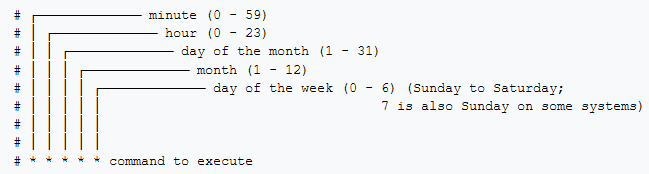
\includegraphics[scale=0.85]{images/cron.png}
    \caption{Source : Wikipédia}
\end{figure}

Certaines versions de cron peuvent tolérer certains standards qui ne sont, quant à eux, pas définis et supportés dans les versions de bases de cron. Ces standards sont utilisables dans les versions de cron sur FreeBSD.
\vspace{0.5cm}

\begin{table}[]
\resizebox{\textwidth}{!}{%
\begin{tabular}{|l|l|l|}
\hline
Standards      & Significations                         & Équivalent  \\ \hline
@yearly        & Une fois par an                        & 0 0 1 1 *   \\ \hline
@annually      & Une fois par an (identique à @yearly)  & 0 0 1 1 *   \\ \hline
@monthly       & Une fois par mois                      & 0 0 1 * *   \\ \hline
@weekly        & Une fois par semaine                   & 0 0 * * 0   \\ \hline
@daily         & Une fois par jour                      & 0 0 * * *   \\ \hline
@midnight      & Une fois par jour (identique à @daily) & 0 0 * * *   \\ \hline
@hourly        & Une fois par heure                     & 0 * * * *   \\ \hline
@every\_minute & Une fois par minute                    & */1 * * * * \\ \hline
@every\_second & Une fois par seconde                   & N/A         \\ \hline
@reboot        & Une fois au démarrage de cron          & N/A         \\ \hline
\end{tabular}%
}
\end{table}
\newpage
\subsection{L'intégration continue}

Dans l'analyse des solutions, une notion importante sera mentionnée : L'intégration continue.
\\
L'intégration continue permet aux créateurs de sites web, d'applications mobiles ou de logiciels de réduire considérablement leur temps passé sur les compilations et tests de paquets.
\\
Cela leur permet de consacrer plus temps au développement de leurs applications.
\\
Ci-dessous, une représentation graphique de l'intégration continue

\begin{figure}[ht]
    \centering
    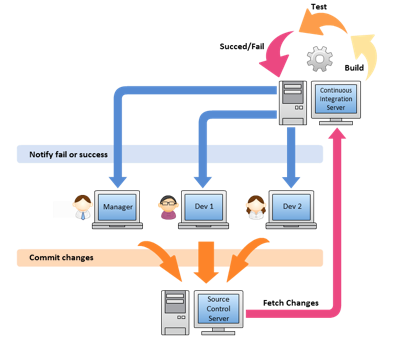
\includegraphics[scale=0.8]{images/IC.png}
    \caption{Intégration continue}
\end{figure}

\newpage
L'intégration continue s'accompagne de 2 autres notions : Le déploiement continu et l'exécution continue.
\\
Ces 2 notions correspondent à un prolongement de l'intégration continue, c'est-à-dire :
\\
\textbf{L'exécution continue ou continuous integration (CI) en anglais} comprends toutes les étapes de l'intégration continue mais en ajoutant les étapes de publication du paquet aux utilisateurs
\\
\textbf{Le déploiement continue ou continuous deployement (CD) en anglais} contient les étapes des 2 notions précédentes en ajoutant l'étape de l'installation automatique du paquets
\\
Ci-dessous, un schéma détaillé de ces différentes notions.
\begin{figure}[ht]
    \centering
    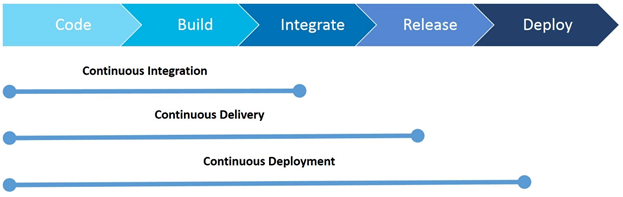
\includegraphics[scale=0.8]{images/IC-plan.png}
    \caption{Notions d'intégrations}
\end{figure}

\newpage
\section{Cron}

\begin{figure}[ht]
    
\includegraphics[scale=0.5]{images/crontab.png}
    \caption{Logo de Crontab}
\end{figure}

\subsection{Présentation}

\textit{Cron est la troncation de crontab, lui-même la troncation de chrono table qui signifie « table de planification » source : Wikipédia}
\vspace{0.5cm}
\\
\textbf{ATTENTION : Cron et Crontab sont 2 programmes différents mais ils ne vont pas l'un sans l'autre. En effet, cron est le planificateur de tâches tandis que Crontab est le programme qui permet d'éditer les fichiers de configuration de cron.}
\vspace{0.5cm}
\\
Les origines de cron se situent dans les systèmes Unix de Berkeley ainsi que AT\&T et a été ensuite développé par Paul Vixie, ce qui fait de lui son auteur original.
\\
Le programme cron à été repris et développé par AT\&T Bell Laboratories, aussi connu sous le nom de Nokia Bell Labs.
\\
Cron est une fonctionnalité native des systèmes Unix. C'est le planificateur de tâches par défaut et intégré à chaque distribution Linux.
\\
Cron est l’ancêtre et l'outil de  planification le plus simple mais aussi le plus accessible pour tout le monde sur Linux
\\
Cron est disponible sous les systèmes Linux, MacOS et FreeBSD sous une interface CLI.
\\
Cron est un daemon (démon), c'est-à-dire que c'est un programme qui s'exécute en arrière plan

\subsection{Historique et versions}
Le programme cron apparaît pour la première en mai 1975, c'est-à-dire, bien avant les distribution Linux que l'on connaît actuellement.
\\
Il est, à l'heure actuelle, maintenu par ces mêmes laboratoires, mais également par des mainteneurs indépendants.

\subsection{Contexte d'utilisation}
Étant un planificateur de tâches, cron est utilisé pour la planification quotidienne, hebdomadaire, mensuelle ou encore annuelle de tâches de maintenances.

\subsection{Fonctionnement}
Cron permet la planification et l'exécution automatique de tâches programmées à l'avance.
\\
Ces tâches sont réglées dans un fichier contenant la commande à exécuter ainsi que l'heure d'exécution.
\\
Le paramétrage d'une tâche est, quant à lui, très simple. Pour automatiser une tâche, il suffit d'écrire dans les fichiers de configuration de cron avec crontab, la commande à exécuter ainsi que l'heure et le jour à laquelle cron doit l'exécuter.
\\
Il est possible de recevoir une notification par mail sur le statut de la tâche, mais cela nécessite l'installation d'un client mail sur la machine.
\\
Ces tâches sont exécutées par l'utilisateur root afin d'éviter les problèmes de droits
\\
En revanche, cron ne permet pas une centralisation des données ou encore une exécution de tâches à distance.
\\
Cron est un programme qui fonctionne uniquement \textbf{en local}

\subsection{Fonctionnalités}
Cron permet une planification de tâches pouvant s'exécuter quotidiennement, hebdomadairement, mensuellement ou encore annuellement. 
\\
Cette fréquence se règle avec des paramètres. Une notification par mail, facultative, peut être également paramétrée.

\subsection{Installation}
Cron ne requiert pas d'installation. Il est cependant possible de l'installé si ce dernier n'est pas présent sur la machine. 
\\
Si l'installation de cron est nécessaire, il suffit de télécharger cron depuis les dépôts via la commande "sudo apt-get install cron".
\\
Cette commande peut varier selon la distribution mais le paquet de cron porte, quant à lui, le même nom.

\subsection{Conclusion}
Cron est un programme simple de planification et d'exécution automatique de tâches. Il est considéré comme étant le "père" des logiciels d'automatisations. Son utilisation simple séduit encore de grands nombres d'adeptes de l'automatisation.
\\
Après 45 ans de service , Cron reste populaire de par sa simplicité et continue de séduire un grand nombre d'utilisateurs à travers le monde.

\section{Jenkins}

\begin{figure}[ht]
    
\includegraphics[scale=0.5]{images/jenkins.png}
    \caption{Logo de Jenkins}
\end{figure}

\subsection{Présentation}

Jenkins est un outil en Open-Source d'intégration continue et d'automatisation de processus
\\
Sorti en 2011, Jenkins est un dérivé de son prédécesseur Hudson, il est présenté comme étant un fork\footnotemark[1] d'Hudson.
\\
Jenkins est également un programme cross-platform disponible sur les systèmes UNIX, Windows et Mac OS. 
\\
Jenkins est hébergé sur la plate forme GitHub, ce qui permet à chaque utilisateur de Jenkins de contribuer à son développement. 
\\
Jenkins est, en majeure partie, amélioré grâce à ses utilisateurs. Ces derniers peuvent participer au développement de Jenkins par la notification de bugs/fonctionnalités manquants ou en rejoignant une équipe de développement de Jenkins. 
\\
Jenkins est développé en JAVA, propose une interface WEB et requiert donc des dépendances JAVA.
\\
La version "Entreprise" de Jenkins est CloudBees.
\\
CloudBees fonctionne, quant à lui, en mode PaaS (Platform as a Service) et supporte le cycle de vie entier d'une application.

\footnotetext[1]{fork : dérivé de ... (trad. litt. : fourchette)}
\subsection{Historique et versions}

Jenkins sort en 2011 et est également disponible sur la plate forme GitHub.
\\
Sa dernière version en date est la 2.204.1 datant du 18 décembre 2019.
\\
Jenkins apparaît suite à la cessation d'Hudson par Oracle à la fondation Eclipse. Jenkins devient en 2011, le successeur d'Hudson.
\\
Contrairement à Jenkins, Hudson est un framework d'intégration continue.
\\
Jenkins est publié sous la licence MIT
\\
Jenkins et Hudson ont été développé par le même développeur : Kohsuke Kawaguchi

\subsection{Contexte d'utilisation}

Jenkins est un logiciel d'intégration continue utilisé pour la compilation automatique de codes sources lors de la création de nouveaux programmes et/ou mises à jours .

\subsection{Fonctionnement}

Jenkins est une application WEB en JAVA qui se déploie de manière autonome dans un conteneur WEB de type Tomcat.
\\
Cependant, Jenkins peut fonctionner sur toutes les plateformes pouvant exécuter une JVM (JAVA Virtual Machine) parmi lesquelles on retrouve Ubuntu/Debian, Windows ou même Mac OS à la seule condition d'avoir les paquets Java correspondants sous peine de rencontrer des problèmes d'exécution ou d'affichage.
\\
Jenkins exécute de manière continue la construction des projets ou "build".
\\ 
Afin que Jenkins puisse permettre l'intégration continue, il exécute les directives de fabrication du logiciel (compilation, assemblage, tests et packaging).
\\
Jenkins peut également exécuter des jobs, soit sur lui-même, soit sur des serveurs distants.
\\
Les jobs construisant les builds, ils peuvent être exécutés sur le serveur Jenkins lui-même ou répartis sur plusieurs machines distantes. Jenkins conserve l'historique de toutes les exécutions des jobs et peut notifier par mail ou par RSS en cas erreur.

\subsection{Fonctionnalités}
Jenkins propose un large panel de fonctionnalités comme exécuter des jobs à distance via SSH, le transfert de fichiers via SCP ou FTP. 
\\
Jenkins peut très bien s'intégrer avec différents gestionnaires de versions, outils de fabrications ainsi que différents outils de suivi d'incidents/bogues. 
\\
Grâce à Jenkins, des outils de contrôle de qualité de cote mais aussi des tests d'intégrations, de performance ou encore des tests de fonctionnement peuvent être effectués.
\\
Jenkins permet également le transfert d'artefacts vers un répertoire.

\subsection{Installation}

Jenkins demande certaines exigences pour permettre son bon fonctionnement.
\\
\vspace{0.5cm}

\textbf{Minimum :}
\begin{itemize}
\item 256 MB de mémoire RAM
\item 1 GB d'espace disque (10 GB sont requis si Jenkins fonctionne dans un conteneur docker
\end{itemize}

\vspace{0.5cm}

\textbf{Recommandé :}
\begin{itemize}
\item 1 GB ou plus de mémoire RAM
\item 50 GB ou plus d'espace disque
\end{itemize}

\vspace{0.5cm}

\textbf{Programmes :}
\begin{itemize}
\item Java : OpenJDK JDK / JRE 8 - 64 bits ou OpenJDK JDK / JRE 11 - 64 bits
\item Navigateur : Dernière version de Google Chrome, Mozilla Firefox, Microsoft Internet Explorer, Microsoft Edge, Apple Safari
\end{itemize}

\vspace{0.5cm}
Un des avantages de Jenkins est qu'il peut être installé sur n'importe quel système d'exploitation. Il peut être installé, soit en programme seul, soit dans un conteneur Docker ou encore via les archives WAR.
\\
\textbf{Linux :}
Pour une installation de Jenkins hors Docker, il suffit de récupérer le répertoire de Jenkins via le terminal qui contient la dernière version de celui-ci. Une fois ce répertoire récupéré, il suffit de l'installer via le terminal.
\\
Les commandes varient selon la distribution utilisée.
\\
Dés lors que l'installation est terminée, il est préférable de vérifier que Jenkins ait bien démarré sur la machine, en utilisant systemctl.
\vspace{0.5cm}
\\
Exemple d'installation sur Ubuntu/Debian :
\begin{lstlisting}
    wget -q -O - https://pkg.jenkins.io/debian/jenkins.io.key | sudo apt-key add -
    sudo sh -c 'echo deb https://pkg.jenkins.io/debian-stable binary/ > \textbackslash /etc/apt/sources.list.d/jenkins.list'
    sudo apt-get update
    sudo apt-get install jenkins
\end{lstlisting}

\vspace{0.5cm}

\textbf{Windows :}
L'installation de Jenkins sur Windows peut se faire de 2 manières :
\begin{itemize}
    \item Sur un conteneur Docker (se référer à la page d'installation contenant les instructions)
    \item En téléchargeant l'installateur et en l'exécutant
\end{itemize}

\vspace{0.5cm}

\textbf{macOS :}
\begin{lstlisting}
    brew install jenkins-lts # Installation de la derniere version
    brew install jenkins-lts@VERSION # Installation d'une version specifique
    brew services start jenkins-lts #  Demarrage des services de Jenkins
    brew services restart jenkins-lts # Redemarrage de Jenkins
    brew upgrade jenkins-lts # Mise a jour
\end{lstlisting}

Jenkins peut être installé de plusieurs manières pour n'importe quel système d'exploitation
\subsection{Conclusion}
Malgré d'énormes ressemblances avec Rundeck, Jenkins est un outil d'intégration continue pour la construction automatique de paquets.

\section{Buildbot}

\begin{figure}[ht]
    
\includegraphics[scale=0.6]{images/buildbot.jpg}
    \caption{Logo de Buildbot}
\end{figure}


\subsection{Présentation}
Buildbot est un framework en Open-Source d'intégration continue
\\
Buildbot est un framework cross-platform et est disponible sur les systèmes Windows et POSIX (Portable Operating System Interface et X signifiant l'héritage UNIX)
\\
Ce framework est présenté comme une alternative au projet de Mozilla : \underline{Tindebox}
\\
Bien qu'il possède d'énormes similitudes avec Jenkins, Buildbot est un framework d'intégration continue développé en Python.
\\
Buildbot se démarque de ses concurrents de par son type mais aussi par sa légèreté ainsi que par la possibilité de pouvoir l'installer sur des systèmes d'exploitations portables.
\\
Buildbot est également disponible sur la plateforme GitHub et permet également aux utilisateurs de contribuer à son développement
\\
Buildbot est distribué sous la licence GPLv2.
\\
Depuis Mars 2013, Buildbot supporte l'intégration SCM avec CVS, Bazaar, Darcs, Subversion, Perforce, Mercurial, Git, Monotone, Repo et Bitkeeper

\subsection{Historique et versions}
La première version de Buildbot est sortie le 26 avril 2003. Sa dernière version est la 2.0.7 et est datée du 27 février 2020.

\subsection{Contexte d'utilisation}
Buildbot est utilisé dans le cadre de l'intégration continue, notamment dans le développement de site Web. De grandes entreprises et de nombreux logiciels utilisent Buildbot parmi lesquels on peut retrouver Mozilla, Chromium, WebKit et bien d'autres.

\subsection{Fonctionnement}
Bien que celui-ci soit un framework, le fonctionnement de Buildbot est similaire à celui de Jenkins.
\\
De la même manière que Jenkins, Buildbot propose une automatisation de la construction de paquets.
\\
Buildbot exécute de manière continue la construction des projets ou "build".
\\ 
Afin que Buildbot puisse permettre l'intégration continue, il exécute les directives de fabrication du logiciel (compilations, assemblages et tests).
\\
De la même manière que Jenkins , Buildbot peut exécuter des jobs, soit sur lui-même, soit sur des serveurs distants.
\\
Les jobs construisant les builds, ils peuvent être exécutés sur le serveur Jenkins lui-même ou répartis sur plusieurs machines distantes. Buildbot conserve l'historique de toutes les exécutions des jobs et peut notifier par mail ou par RSS en cas erreur.

\subsection{Fonctionnalités}
Du point de vue de Buildbot, des applications comme CruiseControl ou Jenkins sont structurées de manière à être prêtes pour l'utilisation
\\
Les autres fonctionnalités sont, quant à elles, identiques à celles proposées par Jenkins.
\\
Il permet aux développeurs d'envoyer leurs codes sur un serveur de contrôle de version sur lequel Buildbot ira rechercher les dernières versions du projet afin de le construire et d'effectuer des tests.
\\
En cas d'erreur ou de réussite, Buildbot notifiera le/les développeur(s) en charge du projet

\subsection{Installation}
Buildbot fonctionne sous le principe de master/worker. Il possède, cependant, quelques exigences : 
\begin{itemize}
    \item Le master fonctionne avec la version 3.5 ou supérieur de Python
    \item Le worker fonctionne avec la version 2.7, 3.5 ou supérieur de Python
\end{itemize}
\vspace{0.5cm}
Tout comme Jenkins, Buildbot peut être installé de différentes manières :
\begin{itemize}
    \item pip install buildbot et pip install buildbot-worker : Installation classique via la commande pip
    \item Après acquisition des Tarballs contenant Buildbot, il suffit de lancer les commandes python setup.py build et python setup.py install
\end{itemize}

\subsection{Conclusion}
Buildbot est un framework d'intégration continue présentant beaucoup de similitudes avec Jenkins. Il reste néanmoins dédié à un certain domaine : le développement Web.

\section{Ansible Tower}

\begin{figure}[ht]
    
\includegraphics[scale=0.4]{images/ansible_tower.png}
    \caption{Logo d'Ansible Tower}
\end{figure}

\subsection{Présentation}
Ansible Tower est un outil d'intégration et de déploiement d'application et/ou de composants divers (comme Nginx ou encore Icinga). 
\\
Il fournit une interface WEB dans laquelle, pourra être gérer Ansible. Par la suite, il pourra créer, supprimer ou encore configurer de nouvelles entités via cette interface.
\\
Ansible Tower est une API en Open Source créée par Red Hat et Ansible. Elle est complètement compatible avec le cloud Amazon AWS (de par sa version Ansible) et le déploiement de conteneur Docker qui permet un bon fonctionnement avec peu de ressources.
\\
De nouvelles versions sont régulièrement disponibles allant de quelques semaines à quelques mois.
\\
Il existe une autre version gratuite appelée AWX qui sert de version beta test pour la version originale TOWER. Cette version gratuite peut être utilisée en entreprise mais ne fournira pas autant de fonctionnalités que la version TOWER.

\subsection{Historique et versions}
Ansible Tower a été créée pour permettre à Ansible (la plateforme de configuration et de gestion d’ordinateurs) d’être utilisée plus facilement sur les équipements informatiques grâce aux API et console web.

\subsection{Contexte d'utilisation}
Ansible Tower est utilisée dans le même cadre d'utilisation que d'autre logiciel d'automatisation. Ansible Tower est l'API de son logiciel principal : Ansible. 
\\
Ansible Tower dispose également d'une console et d'un environnement WEB

\subsection{Fonctionnement}
Ansible Tower va permettre une meilleure sécurité, une adaptabilité et un champ d’application amélioré comparé à une utilisation de Ansible sans cet outil. 
\\
Il permet un accès général au contrôle de la plateforme et gère les identifications SSH. Son inventaire peut être relié à une grande variété de ressources du cloud et de créer des processus complexes. 
\\
Il va créer des logs de suivis des jobs qu'il lance. Il peut être intégré avec un serveur LDAP ou SAML ainsi que d’autres sources d’authentifications. Les outils de lignes de commandes sont facilement utilisables avec Jenkins.

\subsection{Fonctionnalités}
Ansible Tower dispose d'un tableau de bord graphique pour l'utilisateur, la possibilité de planifier des jobs ainsi que de plusieurs API REST. 
\\
A.T\footnotemark[1] permet également une gestion de l'inventaire de manière graphique mais également une intégration d'un système de logging\footnotemark[2] externe.
\footnotetext[1]{Ansible Tower}
\footnotetext[2]{Système de gestion de logs externe}
\\
Cette API dispose d'un système de contrôle d'accès basé sur les rôles.
\\
L'équipe technique de Red-Hat propose un support aux utilisateurs ainsi qu'un portail d'accès pour les clients
\\
Comme certains programmes de gestion et exécution de jobs, Tower permet de suivre les mises à jours du statut des jobs en temps réel mais aussi Tower permet de régler l'ordre d'exécution des playbooks.

\subsection{Installation}
Contrairement aux 3 solutions présentées précédemment, Ansible Tower a, quant à lui, de plus grandes exigences au niveau du système :

\textbf{Systèmes supportés :}
\begin{itemize}
    \item Red Hat Enterprise Linux 8.0 ou supérieur 64-bit (x86) (Ansible Tower 3.5 ou supérieur seulement peut être installé)
    \item Red Hat Enterprise Linux 7.4 ou supérieur 64-bit (x86)
    \item CentOS 7.4 ou supérieur 64-bit (x86)
\end{itemize}

\textbf{Exigences systèmes :}
\begin{itemize}
    \item Dernière version de Google Chrome ou Mozilla Firefox
    \item 2 CPUs minimum
    \item 4 GB de RAM minimum pour l'installation de Tower (pour base de données externe ou une démo d'Ansible Tower via Vagrant)
    \item 20 GB d'espace disque dédié pour les services des noeuds de Tower
    \item 20 GB d'espace disque dédié pour les noeuds contenant une base de données (150 GB+ recommandé)
    \item 64-bit support requis (kernel et runtime)
    \item PostgreSQL version 10 requis pour le fonctionnement d'Ansible Tower 3.6 ou supérieur. Les sauvegardes et restaurations fonctionnent uniquement sur les versions de PostgreSQL supportées par la version installée d'Ansible Tower.
    \item Ansible version 2.2 (minimum) est requise pour utiliser les versions Ansible Tower 3.2 ou supérieur
\end{itemize}

Une fois ces exigences remplies, il suffit de télécharger la dernière version d'Ansible Tower et de l'extraire.
\vspace{0.5cm}
\\
Pour installer ou mettre à jour Tower, il suffit de modifier le fichier d'inventaire se situant dans le dossier ansible-tower-setup-<tower\_version> en remplaçant le numéro de version de la ligne <tower\_version> par le numéro de version tels que 2.4.5 ou 3.0.0

\subsection{Conclusion}
Ansible Tower va permettre une meilleure gestion de ce que propose Ansible ainsi qu'une prise en main plus simple et rapide.

\section{JobScheduler}

\begin{figure}[ht]
    \centering
    
\includegraphics[scale=0.6]{images/jobscheduler.jpg}
    \caption{Logo de JobScheduler}
\end{figure}

\subsection{Présentation}
Développé par "Software- und Organisations-Service GmbH", JobScheduler est un ordonnancer en Open-Source de travaux d'informations et d'automatisations de processus.
\\
Il est distribué sous la licence GPLv2 mais est également disponible sous une licence commerciale pour un support et des services de niveau entreprise.
\\
Ce logiciel est fourni avec plusieurs types d'interfaces : une interface Web, un client graphique ainsi qu'une interface CLI.
\\
JobScheduler est composé de 2 sous programmes : \textbf{JobScheduler Master and JOC\footnotemark[1] Cockpit} et \textbf{JobScheduler Universal Agent}.
\\
JobScheduler Universal Agent est lui même composé de JobScheduler Master et de JobScheduler Agent
\\
Ce programme est présent sur certaines plateformes telles que Windows Server 2008 R2, Windows Server 2012 R2, 2016, Windows 7 et 10, mais également sur Linux RHEL  6, 7 et 8 ainsi que CentOS  6, 7 et 8.

\footnotetext[1]{JOC : JobScheduler Opération Center}

\subsection{Historique et versions}
JobScheduler sort pour la première fois en 2005, la dernière version stable est la 1.13.3 datée du 4 février 2020.
\\
Plusieurs versions majeures ont vues le jour avant la version 1.13.3 : il s'agit des versions 1.9 le 30-04-2015, la 1.10 le 15-09-2015, 1.11 le 20-03-2017 ainsi que la version 1.12 le 21-12-2017.
\\
La première version de la 1.13 est sortie le 29-08-2019

\subsection{Contexte d'utilisation}
Ce logiciel est utilisé pour lancer des fichiers exécutables ainsi que des scripts shells. Il permet également d'exécuter, de manière automatique, des procédures sur des bases de données. 

\subsection{Fonctionnement}
Le type de fonctionnement que propose JobScheduler est le mode SaaS, c'est-à-dire : Software as a Service (Logiciel comme service)
\\
Le fonctionnement de JobScheduler par rapport à ses pairs est différent. En effet, JobScheduler est un ensemble de programmes qui ont tous un rôle différent.
\\
Le programme principal dispose d'une interface Web, d'un client graphique ainsi que d'une interface CLI (\textbf{JOC Cockpit}). C'est depuis ce programme que l'utilisateur dirige toutes les opérations.
\\
Au travers de cette interface, l'utilisateur va envoyer des ordres d'exécutions de jobs aux "Masters".
\\
Les Masters gèrent l'exécution des jobs et orchestrent également les Agents.
\\
JobScheduler Agent est le 3 ème sous-programme, les Agents sont déployés sur les serveurs sur lesquels les programmes et/ou scripts sont exécutés et qui doivent être ordonnancés.
\\
Les informations obtenues par les Masters, à la suite de l'exécution des jobs, sont envoyées à la base de données de JobScheduler afin de pouvoir obtenir un historique des jobs.
\\
JOC Cockpit ainsi que JobScheduler Universal Agent sont disponibles sur seulement 2 plateformes : Windows et Linux
\\
En revanche, ces masters, bien qu'ils soient utilisables sur 2 plateformes, peuvent commander les agents, qui eux sont disponibles pour un plus grands nombres de plateformes.
\\
Les Agents fonctionnent sur les plateformes HP-UX, MacOS, Docker, Raspberry Pi, Solaris, AIX ainsi que toutes autres plateformes.
\\
Les Agents sont utilisables sur n'importe quelle plateforme, du moment que cette dernière supporte une machine virtuelle JAVA.

\subsection{Fonctionnalités}
JobScheduler propose une interface graphique, un client graphique et une interface CLI.
\\
Son mode de fonctionnement étant différent de celui de ses pairs, certaines fonctionnalités changent en fonction du service utilisé.
\\
JobScheduler offre 2 services pour le cloud : Cloud Hosting Service et Cloud Managed Service.
\\
Certaines fonctionnalités entre ces 2 services telles que la planification de jobs ou encore l'accès au JOC Cockpit pour le monitoring des jobs, restent les mêmes.
\\
\textbf{Cloud Hosting Service :}
\begin{itemize}
    \item Mise en place d'une infrastructure de planification
    \item Mise en place d'un système de management des mises à jours et patchs
    \item Accès à des serveurs dédiés via SSH ou SFTP
    \item Accès à JOC Cockpit pour le monotoring et le contrôle des jobs
    \item Intégration du cloud au réseau de l'entreprise
    \item Déploiement des Agents de JobScheduler sur un environnement informatique
    \item Gestion des jobs
    \item Upload des jobs sur des serveurs dédiés via SFTP
    \item Monitoring de l'exécution des jobs
\end{itemize}

\vspace{0.5cm}

\textbf{Cloud Managed Service :}
\begin{itemize}
    \item Mise en place d'une infrastructure de planification
    \item Mise en place d'un système de management des mises à jours et patchs
    \item Accès à JOC Cockpit pour le monotoring et le contrôle des jobs
    \item Intégration du cloud au réseau de l'entreprise
    \item Management des jobs ainsi que des dépendances de jobs par l'équipe de JobScheduler
    \item Monitoring de l'exécution des jobs 24/7
    \item Déploiement des Agents de JobScheduler sur un environnement informatique
    \item Spécification des jobs ainsi que de leurs dépendances
\end{itemize}

\subsection{Installation}
Contrairement aux autres logiciels d'automatisations de processus, JobScheduler n'impose pas une certaine configuration.
\\
Les installateurs sont à télécharger depuis la page des téléchargement de JobScheduler, que ce soit pour Windows ou pour Linux
\\
Il est possible d'installer JobScheduler de manière graphique par l'intermédiaire d'un installateur graphique, ou en ligne de commande.
\\
L'installation graphique n'est valable que pour Windows. Cependant il est possible d'installer JobScheduler sur Windows en ligne de commande via l'invité de commande.
\\
L'installation de JobScheduler sur Linux est exclusivement en ligne de commande et se fait au travers du terminal de commande.
\\
Quelque soit la plateforme sur laquelle JobScheduler doit être installée, il est demandé à l'utilisateur de configurer plusieurs éléments lors de la mise en place.
\vspace{0.2cm}
\\
\textbf{Éléments à configurer :}
\\
\begin{itemize}
    \item Langues disponibles 
    \item Documentation
    \item Licence
    \item Contrat
    \item Répertoire d’installation
    \item Répertoire d’exploitation
    \item Composants
    \item Caractéristiques
    \item Cluster
    \item Messagerie
    \item Envoi de mail
    \item Gestionnaire de bases de données
    \item Base de données
    \item Crontable (optionnel)
    \item Installation
    \item Journal 
    \item Statut
\end{itemize}

\vspace{0.5cm}
\textbf{L'installation silencieuse :}
L'installation silencieuse est présente sur Windows, sous la forme de fichier ayant l'extension .msi, ainsi que sur Linux.
\\
L'installation silencieuse sur Linux consiste à remplir un formulaire pour le programme en question
\\
Ce formulaire, une fois rempli, permettra de générer un fichier d'installation silencieuse.
\\
Pour procéder à l'installation avec ce fichier, il suffit, simplement, de l'exécuter
\\
L'installation silencieuse est une étape facultative mais qui présente de nombreux avantages.
\\
Pour JobScheduler, il est possible, sur Linux, de l'installer par l'intermédiaire de l'installation silencieuse.
\\
Si le fichier d'installation silencieuse n'est pas généré, il est possible de configurer JobScheduler directement dans son fichier d'installation
\\
Le fichier d'installation silencieuse a le même rôle que l'installateur graphique, mais de manière plus compacte.
\\
L'installation via le cmd ou le terminal se fera de manière un peu plus condensée que la version graphique.
\\
Néanmoins les éléments à configurer restent les mêmes
\\
La génération d'un fichier d'installation silencieuse se fait par l'intermédiaire d'une instance Arii

\subsection{Conclusion}
JobScheduler est un ordonnanceur de tâches proposant des services de gestion pour les bases de données et les clouds. Il est modulaire et possède un fonctionnement simple


\section{Rundeck}

\begin{figure}[ht]
    
\includegraphics[scale=0.8]{images/rundeck.jpg}
    \caption{Logo de Rundeck}
\end{figure}

\subsection{Présentation}

Dans le cadre de notre projet, nous avons choisi la solution Rundeck.
\\
Rundeck est un logiciel Open-Source d'automatisation de gestion de parc informatique. Rundeck est définit comme un orchestrateur de tâches. 
\\
Sorti en 2011, il dispose d'une variante entreprise appelé "Rundeck Entreprise" permettant la gestion d'un parc informatique de plus grande envergure. 
\\
Rundeck est également un logiciel cross-platform disponible pour les systèmes UNIX, Windows et Mac OS. 
\\
Rundeck est hébergé sur la plate forme de développement GitHub, ce qui permet à chaque utilisateur de Rundeck de contribuer à son développement. 
\\
Rundeck est, en majeure partie, amélioré grâce à ses utilisateurs. Ces derniers peuvent participer au développement de Rundeck par la notification de bugs/fonctionnalités manquants ou en rejoignant une équipe de développement de Rundeck. 
\\
Rundeck est développé en JAVA et propose une interface WEB (requiert les paquets JAVA), une interface CLI (Command-Line Interface) ainsi qu'une API REST.

\subsection{Historique et versions}

Rundeck est apparu en 2011 suite à la demande de plus en plus forte du besoin de pouvoir administrer tous les serveurs d'un parc informatique depuis un seul serveur d'administration central.
\\
La dernière version en date est la version 3.2.0 datant du 10 février 2020.
\\
Rundeck est diffusé sous la licence Apache Software 2.0

\subsection{Contexte d'utilisation}

Rundeck est, parmi un large panel de logiciel d'automatisation, un des plus utilisé lorsque l'utilisateur souhaite automatiser la gestion d'un parc informatique depuis une seule machine physique.
\\
Il est notamment utilisé avec Ansible, cette combinaison présentant de nombreux avantages.

\subsection{Fonctionnement}

Rundeck permet l'exécution de tâches et/ou jobs sur des serveurs distants via une connexion SSH. Rundeck fonctionne sur des réseaux privés où les machines possèdent des adresses IP statiques. 
\\
Les adresses IP dynamiques des serveurs distants peuvent causer des conflits d'IP et de clés SSH sur le serveur de Rundeck.
\\
Rundeck est également basé sur le principe maître/esclave (master/slave) : La machine où se trouve l'application Rundeck est le maître tandis que le serveur distant est l'esclave. 
\\
De plus, Rundeck montrera un meilleur fonctionnement si celui-ci est installé sur une distribution orientée serveur telle que CentOS. 
\\
Par défaut, Rundeck écoute sur le port 4440 (http) mais peut également écouter sur le port 4443 (https)
\\
Cependant, Rundeck peut être installé sur d'autres distributions telles qu'Ubuntu, Debian ou même Windows à la seule condition d'avoir les paquets Java correspondants sous peine de rencontrer des problèmes d'exécution ou d'affichage.
\\
Rundeck, par défaut, fonctionne avec sa propre base de données, une interface WEB ainsi qu'un compte administrateur dont les identifiants sont "admin" pour le nom d'utilisateur et "admin" pour le mot de passe.
\\
Toutefois, la base de données embarquée de Rundeck est dépourvue de systèmes de sécurité optimale, il est recommandé d'utiliser une base de données spécifique.
\\
Cette base de données est de type H2, c'est à dire que c'est une base de données de très petites taille et écrite en JAVA 

\subsection{Fonctionnalités}

Rundeck possède une grande gamme de fonctionnalités qui permettent à l'utilisateur de Rundeck, une gestion optimale d'un parc informatique. Rundeck met à disposition un choix de plus de 1000 plugins de nature diverse et variée. 
\\
Rundeck propose également diverses fonctionnalités notamment l'exécution de commandes/tâches à distance
\\
Rundeck est également très modulable. En effet, Rundeck utilise une base de données embarquée pour l'enregistrement de données telles que les jobs, les clés SSH et les utilisateurs qui ont accès à Rundeck.

\subsection{Installation}
L'installation de Rundeck est très simple, il est recommandé de l'installer sur CentOS afin de pouvoir utiliser Rundeck de manière optimale. Il est également possible d'installer ce programme sur Windows. 
\\
\textbf{Étant au centre de notre projet, la procédure d'installation de Rundeck se trouve plus bas dans le document, au point 15.2 ainsi que dans la notice}

\subsection{Conclusion}
Rundeck est un orchestrateur de tâches permettant la maintenances de serveurs à distance. Il peut être couplé avec une base de données externe et également à d'autres programmes tel qu'Ansible.

\newpage
\section{Tableaux synthétiques}
Ces tableaux comparatifs présentent les diverses solutions envisagées. Les critères sont organisés par catégorie afin que cela soit plus lisible. Des informations complémentaires pourraient apparaître dans ces tableaux
\vspace{0.5cm}
\\
\textbf{Années de sortie :}

\vspace{0.5cm}

\begin{center}
\begin{tabular}{|l|l|}
\hline
Solutions     & Années de sortie \\ \hline
Cron          & 1975             \\ \hline
Jenkins       & 2011             \\ \hline
Buildbot      & 2003             \\ \hline
Ansible Tower & 2015             \\ \hline
JobScheduler  & 2005             \\ \hline
Rundeck       & 2011             \\ \hline
\end{tabular}
\end{center}

\vspace{0.5cm}

\textbf{Installation :}
Les pré-requis caractérisent une configuration matérielle et logicielle minimum pour installer le programme
\vspace{0.5cm}
\\
\begin{center}
\begin{tabular}{|l|l|l|}
\hline
Solutions     & Pré-requis & Plateforme                 \\ \hline
Cron          & Non        & Linux, MacOS               \\ \hline
Jenkins       & Oui        & Tous OS                    \\ \hline
Buildbot      & Oui        & POSIX, Windows             \\ \hline
Ansible Tower & Oui        & Windows, Linux, Linux-like \\ \hline
JobScheduler  & Oui        & Windows, Linux, Linux-like \\ \hline
Rundeck       & Oui        & Windows, Linux, Linux-like \\ \hline
\end{tabular}
\end{center}

\vspace{0.5cm}

\textbf{Cadre d'utilisation :}
Un résumé très bref sur la nature et le rôle de chaque solution
\vspace{0.5cm}
\\
\begin{center}
\begin{tabular}{|l|l|l|}
\hline
Solutions     & Type      & Rôle / Utilisation         \\ \hline
Cron          & Daemon    & Planificateur de tâches    \\ \hline
Jenkins       & Programme & Intégration continue       \\ \hline
Buildbot      & Framework & Intégration continue (web) \\ \hline
Ansible Tower & API       & Planificateur de tâches    \\ \hline
JobScheduler  & Programme & Planificateur de tâches    \\ \hline
Rundeck       & Programme & Planificateur de tâches    \\ \hline
\end{tabular}
\end{center}

\vspace{0.5cm}

\textbf{Administration :}
Interface : type d'interface 
\vspace{0.2cm}
\\
\textbf{BDD :} Base de données pré-intégré et/ou possibilité d'en intégrer
\vspace{0.2cm}
\\
\textbf{Extensible :} Extension du programme grâce à des plugins
\vspace{0.5cm}
\\
\begin{center}
\begin{tabular}{|l|l|l|l|}
\hline
Solutions     & Interface & BDD & Extensible \\ \hline
Cron          & CLI       & Non & Non        \\ \hline
Jenkins       & Graphique & Non & Oui        \\ \hline
Buildbot      & Graphique & Oui & Oui        \\ \hline
Ansible Tower & Graphique & Oui & Oui        \\ \hline
JobScheduler  & Graphique & Oui & Oui        \\ \hline
Rundeck       & Graphique & Oui & Oui        \\ \hline
\end{tabular}
\end{center}

\vspace{0.5cm}

\textbf{Gestion :}

\begin{center}
\begin{tabular}{|l|l|l|l|}
\hline
Solutions     & Suivi des jobs  & Logs & Stockage des logs   \\ \hline
Cron          & Via logs        & Oui  & Machine locale      \\ \hline
Jenkins       & Après exécution & Oui  & Machine Locale      \\ \hline
Buildbot      & Après exécution & Oui  & BDD                 \\ \hline
Ansible Tower & En temps réel   & Oui  & Machine Locale      \\ \hline
JobScheduler  & En temps réel   & Oui  & Machine Locale      \\ \hline
Rundeck       & En temps réel   & Oui  & BDD, Machine Locale \\ \hline
\end{tabular}
\end{center}
\vspace{0.5cm}
\textbf{LDAP :}
Possibilité de mettre en place un système d'authentification via un annuaire LDAP
\vspace{0.2cm}
\\
\textbf{Plugin :} requiert l'installation d'un plugin
\vspace{0.2cm}
\\
\textbf{Pré-intégré :} Pas de plugins, spécification des adresses des annuaires dans les fichiers de configuration et/ou depuis l'interface graphique
\vspace{0.5cm}
\\
\begin{center}
\begin{tabular}{|l|l|l|}
\hline
Solutions     & Connecteur LDAP & Intégration \\ \hline
Cron          & Non             & Aucune      \\ \hline
Jenkins       & Oui             & Plugin      \\ \hline
Buildbot      & Oui             & Plugin      \\ \hline
Ansible Tower & Oui             & Pré-intégré \\ \hline
JobScheduler  & Oui             & Pré-intégré \\ \hline
Rundeck       & Oui             & Pré-intégré \\ \hline
\end{tabular}
\end{center}

\vspace{0.5cm}

\textbf{Autres :}
Officiel : Support fourni par l'équipe créatrice du programme
\vspace{0.2cm}
\\
\begin{center}
\begin{tabular}{|l|l|l|}
\hline
Solutions     & Support & Type          \\ \hline
Cron          & Oui     & Communautaire \\ \hline
Jenkins       & Oui     & Officiel      \\ \hline
Buildbot      & Oui     & Officiel      \\ \hline
Ansible Tower & Oui     & Officiel      \\ \hline
JobScheduler  & Oui     & Officiel      \\ \hline
Rundeck       & Oui     & Officiel      \\ \hline
\end{tabular}
\end{center}

\section{Mise en place de Rundeck}
\subsection{Environnement de travail}
Dans le cadre de notre projet, nous avons choisit un environnement de travail sous Linux ainsi que l'utilisation de plusieurs outils de virtualisation tels que Vagrant, Oracle VirtualBox.
\\
L'intérêt d'utiliser Oracle VirtualBox pour mettre en place cette infrastructure est qu'il présentera plus de facilité à s'installer sur des machines hôtes sous Linux
\\
Notre infrastructure de travail et de démonstration se fait à l'aide 4 machines virtuelles, mais peut cependant être étendu à un nombre plus grand de machines virtuelles. L'unique contrainte étant les performances des machines hôtes.
\\
\vspace{0.5cm}
\\
\textbf{Infrastructure :}
\begin{itemize}
    \item Machine virtuelle \textbf{rundeck} sous CentOS
    \item Machine virtuelle \textbf{web} sous Debian
    \item Machine virtuelle \textbf{mail} sous Debian
    \item Machine virtuelle \textbf{nfs} sous Debian
\end{itemize}
\vspace{0.5cm}
\textbf{Informations relatives à chaque machine virtuelle :}
\vspace{0.5cm}
\\
\textbf{Rundeck :} 
\\
Le système d'exploitation choisit est CentOS de par son optimisation pour les serveurs. Cette VM est appelée "Rundeck" du même nom que l'outil d'orchestration installé sur cette dernière. Cette VM est la "VM Maître" étant donné qu'elle supervise et gère toutes les autres VMs qui se trouvent sous son autorité. Cette machine virtuelle est générée grâce à une boxe Vagrant 
\\
\vspace{0.5cm}
\\
\textbf{web :}
Cette machine virtuelle joue le rôle d'un serveur web et est installée avec un système Debian GNU/Linux ainsi que tous les composants et paquets requis pour assurer le bon fonctionnement d'un serveur web simple. Cette VM est générée grâce à une box Vagrant 
\\
\vspace{0.5cm}
\\
\textbf{mail :}
Cette machine virtuelle joue le rôle d'un serveur mail et machine est installée avec un système Debian GNU/Linux ainsi que tous les composants et paquets requis pour assurer le bon fonctionnement d'un serveur mail. Cette VM est générée grâce à une box Vagrant 
\\
\vspace{0.5cm}
\\
\textbf{nfs :}
Cette machine virtuelle constitue un point de montage afin de pouvoir partager des fichiers entre chaque machine et est installée avec un système Debian GNU/Linux ainsi que tous les composants et paquets requis pour assurer le bon fonctionnement d'un point de montage de partage de fichiers. Cette VM est générée grâce à une box Vagrant 

\subsection{Installation}
\subsubsection{Exigences système}

\begin{itemize}
    \item Linux: Distributions récentes conseillées pour un fonctionnement optimal
    \item Windows : XP, Server et supérieures (Distributions récentes conseillées)
    \item Mac : OS X 10.4 ou supérieure
\end{itemize}

\vspace{0.5cm}

Accès root (ou administrateur) non requis; création d'un compte utilisateur dédié conseillé par Rundeck 

\vspace{0.5cm}

\textbf{Informations complémentaires fournies par Rundeck}
\begin{itemize}
    \item OS Supportées : Red Hat Enterprise Linux - CentOS - Ubuntu/Debian - Windows Server
    \item Version courante et supportée de Mozilla Firefox ou Google Chrome
    \item 2 CPUs (2 CPUs par membres)
    \item 4 GB de mémoire RAM minimum (taille variable en fonction de la taille du parc)
    \item 20 GB d'espace disque minimum (taille variable en fonction de la taille du parc)
    \item Base de données : Mysql - MariaDB - Postgre - Oracle
    \item Stockage des logs : Système de fichier - Stockage S3
    \item Amazon EC2 : Instance m3.medium ou plus grand (dépend du nombres d'hôte) 
\end{itemize}

\vspace{0.5cm}

La version 1.8 de JAVA est également requise
\subsubsection{Windows}

\subsubsection{Linux}

L'installation de Rundeck sous Linux est très simpliste. Afin d'obtenir un fonctionnement optimal, Rundeck a été mis en place sous CentOS. Son installation est composée des étapes suivantes : 

\vspace{0.5cm}

\begin{lstlisting}
    sudo yum -y install java-1.8.0-openjdk java-1.8.0-openjdk-devel -y # Installation de la version de Java requise
    sudo rpm -Uvh http://repo.rundeck.org/latest.rpm # Recuperation de la derniere version de Rundeck
    sudo yum -y install rundeck # Installation de Rundeck
\end{lstlisting}

\subsection{Configuration}
\subsubsection{Arborescence}
Les fichiers de configuration de Rundeck sont répartis de manière à pouvoir se repérer dans sa configuration, c'est-à-dire qu'ils sont stockés dans le répertoire /etc/rundeck tandis que les fichiers de configurations propres aux tâches/jobs sont stockés dans le répertoire /var/lib/rundeck. 
\\
Ci-dessous, la disposition DEB/RPM :
\newpage
\begin{forest}
  for tree={
    font=\ttfamily,
    grow'=0,
    child anchor=west,
    parent anchor=south,
    anchor=west,
    calign=first,
    edge path={
      \noexpand\path [draw, \forestoption{edge}]
      (!u.south west) +(7.5pt,0) |- node[fill,inner sep=1.25pt] {} (.child anchor)\forestoption{edge label};
    },
    before typesetting nodes={
      if n=1
        {insert before={[,phantom]}}
        {}
    },
    fit=band,
    before computing xy={l=15pt},
  }
[/etc/rundeck/
  [admin.aclpolicy]
  [apitoken.aclpolicy]
  [artifact-repositories.yaml]
  [cli-log4j.properties]
  [framework.properties]
  [jaas-loginmodule.conf]
  [profile]
  [project.properties]
  [realm.properties]
  [rundeck-config.properties]
  [rundeckpro-licence.key]
  [ssl 
    [ssl.properties]
    [keystore]
    [truststore]
  ]
  [system-job\_reader\.aclpolicy\_template]
  [system-job\_runner\.aclpolicy\_template]
  [system-job\_viewer\.aclpolicy\_template]
  [system-job\_writer\.aclpolicy\_template]
  [system-project\_admin\.aclpolicy\_template]
]
\end{forest}

\newpage
\begin{forest}
  for tree={
    font=\ttfamily,
    grow'=0,
    child anchor=west,
    parent anchor=south,
    anchor=west,
    calign=first,
    edge path={
      \noexpand\path [draw, \forestoption{edge}]
      (!u.south west) +(7.5pt,0) |- node[fill,inner sep=1.25pt] {} (.child anchor)\forestoption{edge label};
    },
    before typesetting nodes={
      if n=1
        {insert before={[,phantom]}}
        {}
    },
    fit=band,
    before computing xy={l=15pt},
  }
  [/var/lib/rundeck
  [bootstrap]
  [cli]
  [data]
  [libext]
  [logs]
  [projects]
  [repository]
  [var]
  [work]
]
\end{forest}
\vspace{0.5cm}
\\
Ci-dessous, la disposition de l'interface de Rundeck :
\vspace{0.5cm}
\\
\vspace{0.5cm}
\begin{forest}
  for tree={
    font=\ttfamily,
    grow'=0,
    child anchor=west,
    parent anchor=south,
    anchor=west,
    calign=first,
    edge path={
      \noexpand\path [draw, \forestoption{edge}]
      (!u.south west) +(7.5pt,0) |- node[fill,inner sep=1.25pt] {} (.child anchor)\forestoption{edge label};
    },
    before typesetting nodes={
      if n=1
        {insert before={[,phantom]}}
        {}
    },
    fit=band,
    before computing xy={l=15pt},
  }
  [\$RDECK\_BASE/etc/
  [admin.acmpolicy]
  [apitoken.aclpolicy]
  [cli-log4j.properties]
  [framework.properties]
  [preferences.properties]
  [profile]
  [profile.bat]
  [project.properties]
]
\end{forest}
\\
\vspace{0.5cm}
\\
\begin{forest}
  for tree={
    font=\ttfamily,
    grow'=0,
    child anchor=west,
    parent anchor=south,
    anchor=west,
    calign=first,
    edge path={
      \noexpand\path [draw, \forestoption{edge}]
      (!u.south west) +(7.5pt,0) |- node[fill,inner sep=1.25pt] {} (.child anchor)\forestoption{edge label};
    },
    before typesetting nodes={
      if n=1
        {insert before={[,phantom]}}
        {}
    },
    fit=band,
    before computing xy={l=15pt},
  }
  [\$RDECK\_BASE/server/config/
  [artifact-repositories.yaml]
  [jaas-loginmodule.conf]
  [log4j.properties]
  [realm.properties]
  [rundeck-config.properties]
  [ssl.properties]
]
\end{forest}
\\
\vspace{0.5cm}
\\
Dans le cadre de notre projet, nous avons appliqué une configuration simple, impliquant les fichiers de configurations suivants :
\begin{itemize}
    \item /etc/rundeck/framework.properties
    \item /etc/rundeck/realm.properties
    \item /etc/rundeck/rundeck-conf.properties
\end{itemize}
\vspace{0.5cm}

\textbf{Informations relatives à chaque onglet :}
\\
\vspace{0.5cm}
\\
\textbf{framework.properties :}
\\
Ce fichier contient diverses informations : Les informations de connexion au serveur Rundeck, l'emplacement des fichiers d'installations ainsi que l'exécuteur SSH et Copier de fichiers par défaut
\\
\textbf{Définition des propriétés de connexion à l'interface Web :} nom du serveur, nom de l'hôte, le port ainsi que l'URL
\\
\textbf{Définition des emplacements des fichiers d'installations :} Stockage des logs, projets, fichiers temporaires etc...
\\
Définition des emplacements des clés SSH ainsi que du temps de connections avant le "timeout"
\vspace{0.2cm}
\\
\textbf{rundeck-conf.properties :}
\\
Ce fichier permet de définir les méthodes de stockages, chiffrement des fichiers ainsi que les niveaux de logs.
\\
\vspace{0.2cm}
\\
\textbf{realm.properties :}
\\
Fichier contenant identifiants, mots de passe et droits de chaque utilisateurs.
\\
Seulement 4 droits sont disponibles : job-runner (peut lancer des jobs), job-writer (peut créer des jobs), job-reader(peut lire les jobs), job-viewer(peut voir les jobs)

\subsubsection{Interface de connexion}
Rundeck est fourni, par défaut, avec une interface web dont l'URL est : 
\\
\underline{\url{http://localhost:4440}}
\vspace{0.2cm}
\\
Cette URL peut, toutefois être modifiée, en éditant les fichiers \textit{framework.properties} et \textit{rundeck-config.properties}.
\\
Le paramètre \textit{framework.rundeck.url} contient l'URL de base de Rundeck et peut être remplacée par une adresse au choix.
\\
Lors de la première utilisation de Rundeck suivant son installation, les identifiants de connexion par défaut son \textit{admin} pour l'"username" et \textit{admin} pour le mot de passe.
\\
Ces identifiants peuvent être changés en éditant le fichier \textit{realm.properties}
\\
Des comptes utilisateurs peuvent être également ajoutés depuis ce même fichier
\\
\begin{figure}[ht]
    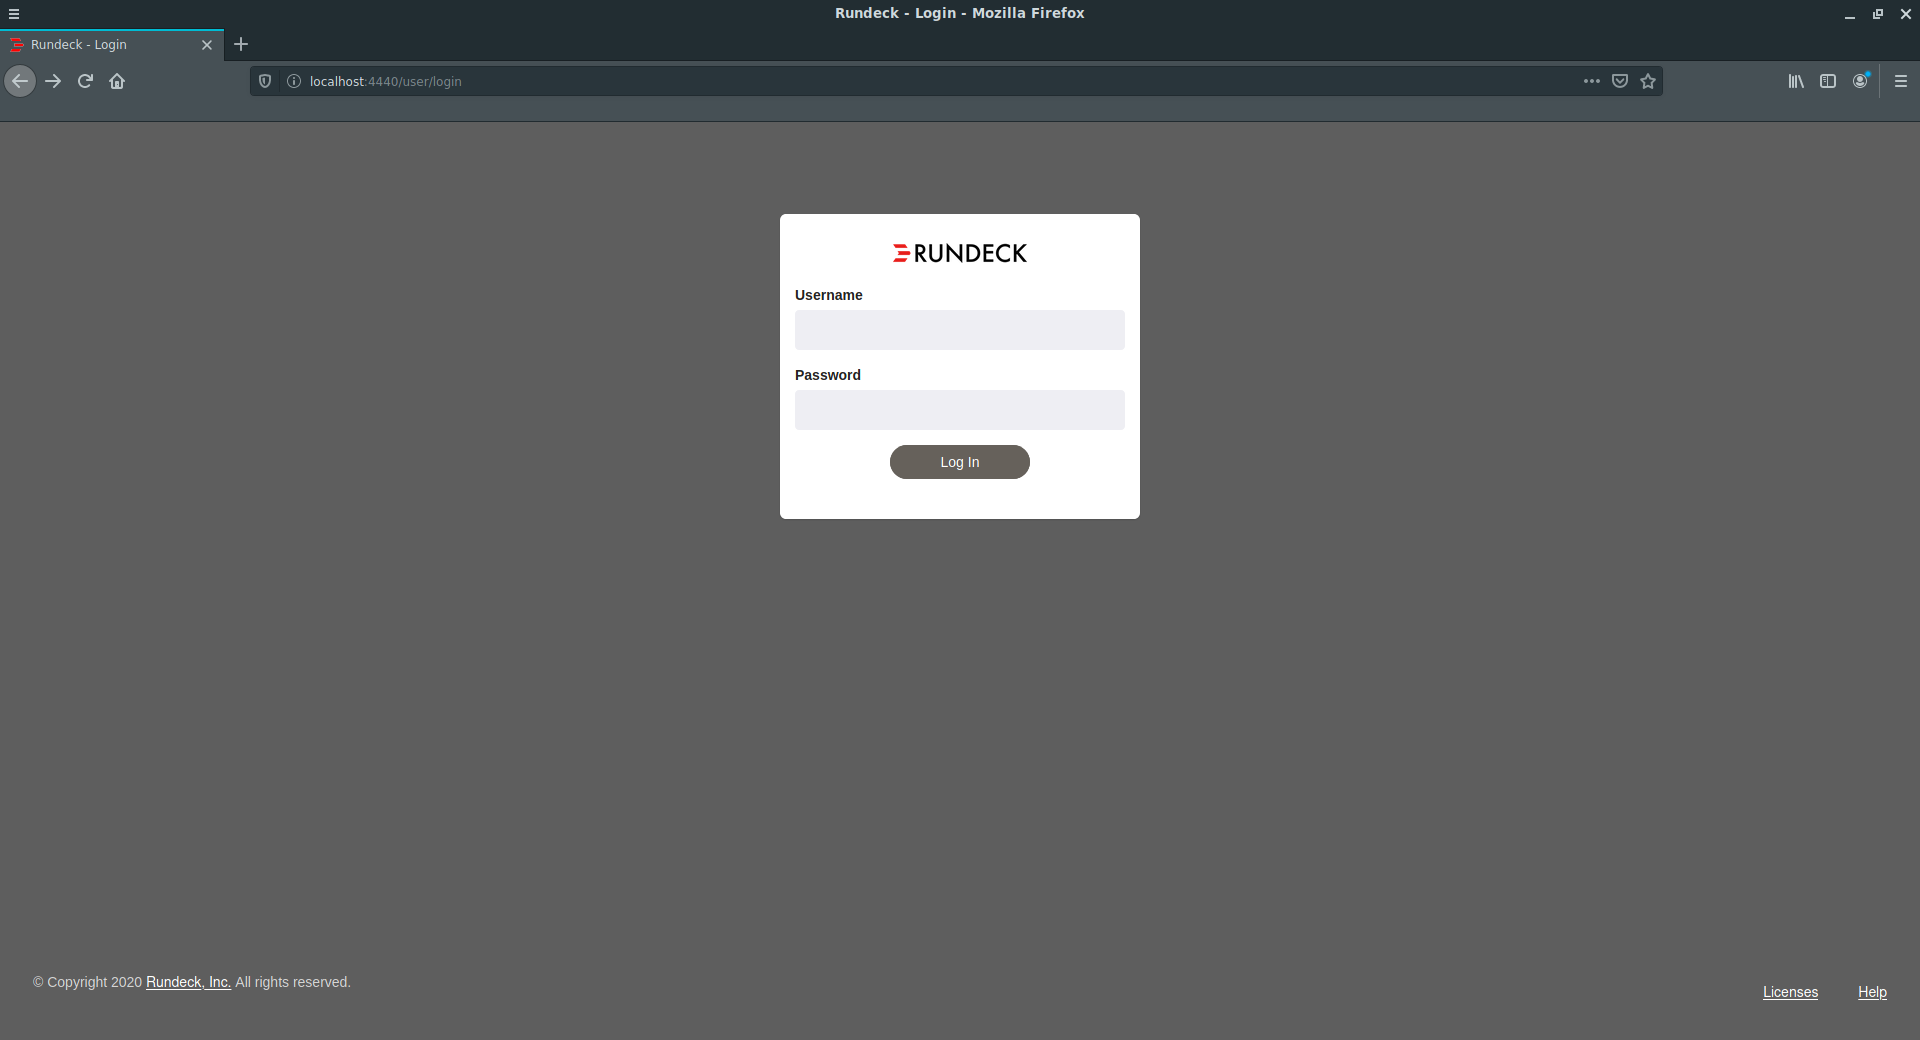
\includegraphics[scale=0.23]{images/connexion.png}
    \caption{Interface de connexion}
\end{figure}
\\
\textit{Username : admin}
\\
\textit{Password : admin}

\subsubsection{Création d'un projet}
La particularité de Rundeck est de pouvoir fonctionner sous forme de projet. Cette fonctionnalité est native à Rundeck et est aussi indispensable.
\\
En effet, les projets permettent de gérer plusieurs parcs informatiques d'une même entreprise depuis une seule et unique machine.
\\
\begin{figure}[ht]
    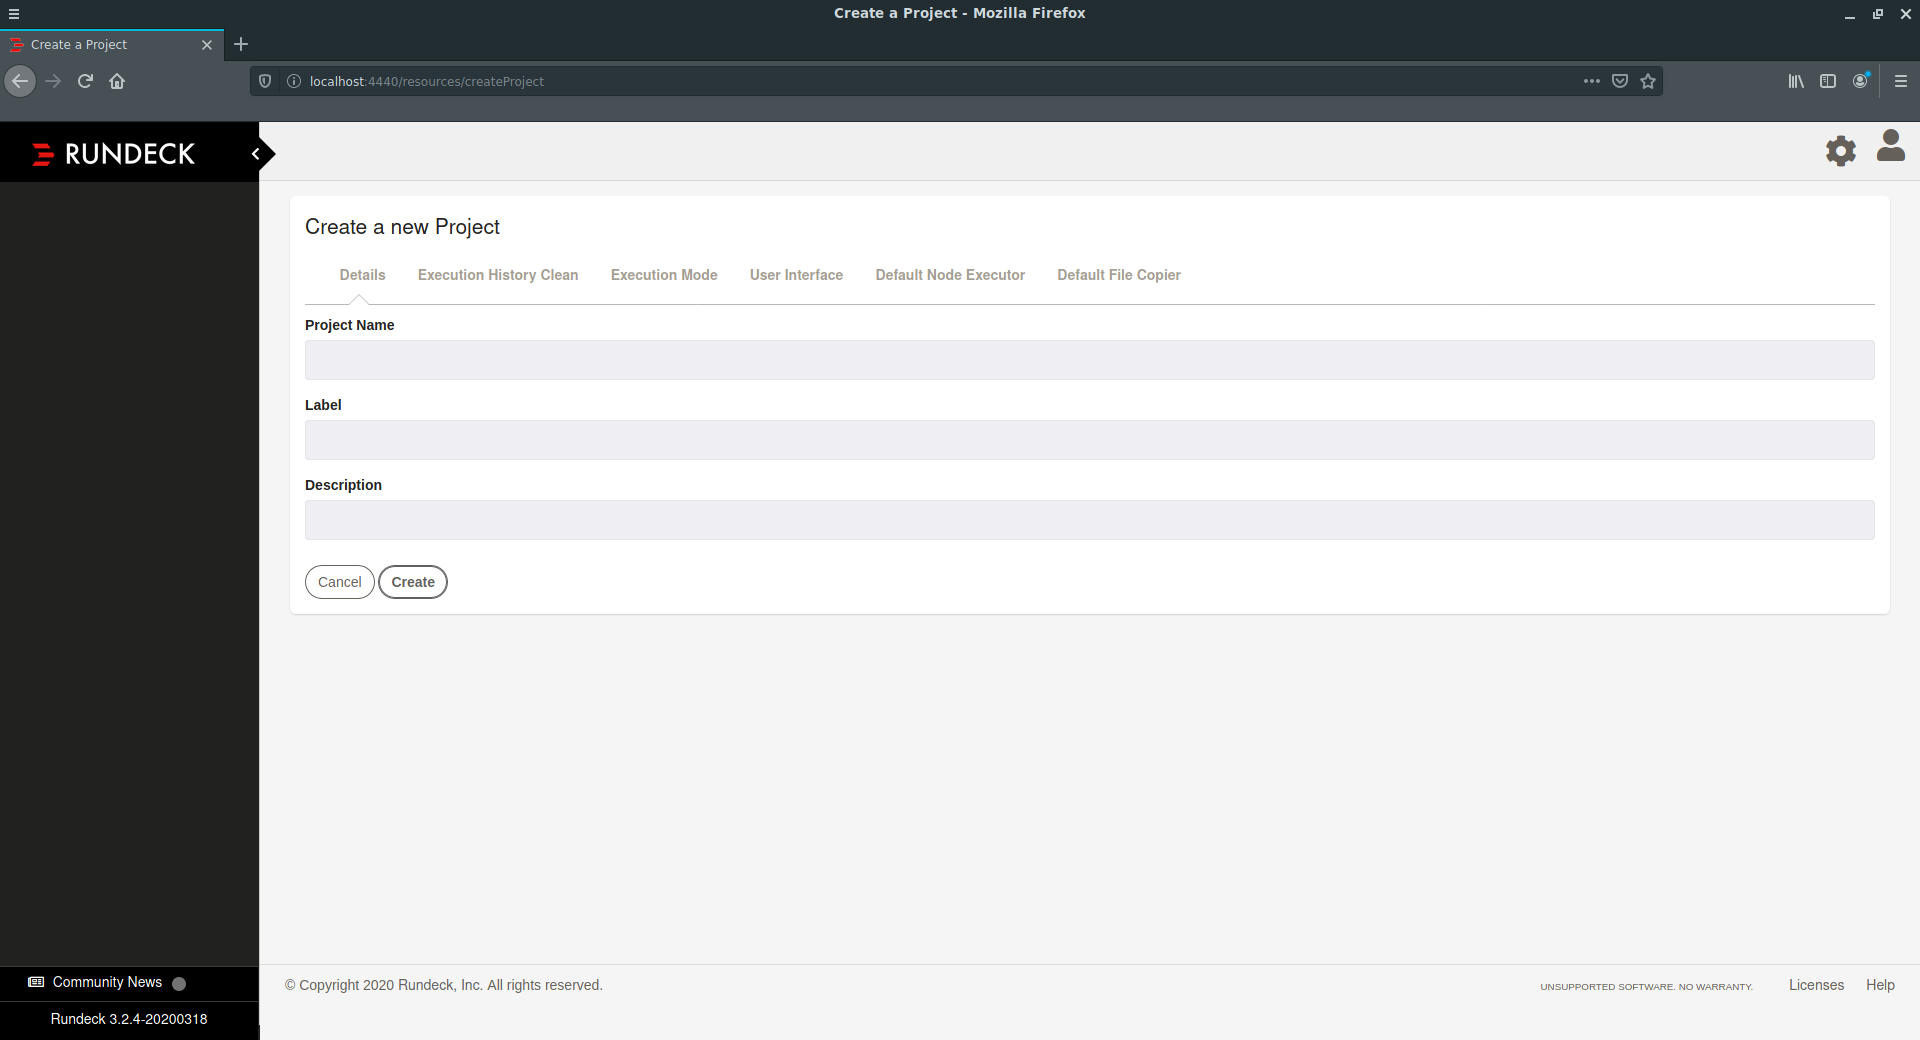
\includegraphics[scale=0.23]{images/project.png}
    \caption{Interface de connexion}
\end{figure}
\\
Lors de la création du projet, plusieurs onglets sont mis à disposition afin de permettre une configuration complète d'un projet
\\
\begin{itemize}
    \item Les détails du jobs \textbf{"Details"}
    \item Nettoyage automatique de l'historique d'exécution \textbf{"Execution History Clean"}
    \item Paramètres d'exécution et planification \textbf{"Execution Mode"}
    \item Personnalisation de l'interface utilisateur \textbf{"User Interface"}
    \item Méthode par défaut d'exécution sur un noeud \textbf{"Default Node Executor"}
    \item Méthode par défaut de copie de fichier sur un node \textbf{"Default File Copier"}
\end{itemize}
\vspace{0.5cm}
\textbf{Informations relatives à chaque onglet :}
\\
\vspace{0.5cm}
\\
\textbf{Onglet "Details" :}
\\
L'utilisateur peut définir, depuis cet onglet, le nom ainsi qu'une courte description du projet
\\
\vspace{0.2cm}
\\
\textbf{Onglet "Execution History Clean" :}
\\
\textit{trad : Nettoyage de l'historique d'exécution}
\\
Cet onglet permet de régler le/les fréquences de nettoyage automatiques des exécutions. Ce nettoyage peut être activé ou désactivé à la demande de l'utilisateur.
\\
Des valeurs par défaut sont imposées par Rundeck telle que le nombre de jours que l'on souhaite garder l'historique (ex: Rundeck supprimera l'historique au bout de 60 jours).
\\
Rundeck propose un nombre d'exécution minimum fixé à 50 exécutions, une taille maximum de l'historique limitée à 500Mo ainsi que la possibilité de paramétrer via \textbf{une expression de type cron} le nettoyage automatique de l'historique.
\\
Ces valeurs sont les valeurs par défaut imposées par Rundeck mais peuvent être modifiées par l'utilisateur de Rundeck.
\\
\vspace{0.2cm}
\\
\textbf{Onglet "Execution Mode" :}
\\
\textit{trad : Mode d'exécution}
\\
Cet onglet permet d'activer/désactiver l'exécution des jobs, des commandes ad-hoc ainsi que la planification des jobs et commandes ad-hoc.
\\
\vspace{0.2cm}
\\
\textbf{Onglet "User Interface" :}
\\
\textit{trad : Interface utilisateur}
\\
Depuis cet onglet, un README ainsi qu'un MOTD ("Message Of The Day") peuvent afficher sur certaines pages lorsqu'un utilisateur de Rundeck se connecte à l'interface
\\
\vspace{0.2cm}
\\
\textbf{Onglet "Default Node Executor" :}
\\
\textit{trad : Exécuteur de node par défaut }
\\
Par défaut, Rundeck règle l'exécuteur sur SSH, c'est-à-dire que les jobs/commandes seront exécutés via SSH. 
\\
Cette méthode peut toutefois être changée si Rundeck possède des machines d'une autre distribution que Linux sous son contrôle. 
\\
Plusieurs méthodes sont mis à disposition par Rundeck et d'autres méthodes peuvent être téléchargées depuis la liste des plugins si la méthode demandée par l'administrateur ne se trouve pas dans la liste fournie par Rundeck
\\
Si des clés SSH et passphrases sont stockées directement sur Rundeck, il est possible de spécifier les chemins de fichiers afin de permettre l'accès via ces protocoles
\\
\vspace{0.2cm}
\\
\textbf{Onglet "Default File Copier" :}
\\
\textit{trad : Copier de fichier par défaut}
\\
Même principe que l'onglet précèdent, celui-ci permet de modifiée l'utilitaire de transfert de fichiers d'une machine à une autre via Rundeck.
\\
Plusieurs méthodes sont mis à disposition par Rundeck et d'autres méthodes peuvent être téléchargées depuis la liste des plugins si la méthode demandée par l'administrateur ne se trouve pas dans la liste fournie par Rundeck
\\
Si des clés SSH et passphrases sont stockées directement sur Rundeck, il est possible de spécifier les chemins de fichiers afin de permettre l'accès via ces protocoles

\subsubsection{Configuration du stockage}

Rundeck propose plusieurs méthodes de stockage :
\vspace{0.2cm}
\\
Méthodes de stockage :
\begin{itemize}
    \item Base de données embarquée
    \item Base de données "spécifique"
    \item Système de fichiers
\end{itemize}

\vspace{0.2cm}
L'emplacement des données peut être sur le système de fichiers de la machine, dans une base de données (spécifique ou celle fournit par Rundeck) ou encore sur un système de stockage externe. Un plugin pour le stockage externe sera requis.*
\\
\vspace{0.2cm}
\\
Rundeck fournit également 2 implémentions possibles :
\begin{itemize}
    \item filesystem : stockage local des données
    \item db - stockage dans une base de données
\end{itemize}
\vspace{0.2cm}
Dans notre cas, nous avons fait appel à la base de données embarquée de Rundeck. L'utilisation d'une base de données spécifique est également fortement recommandée par Rundeck.
\\
La base de données de Rundeck est uniquement réservée pour tester de ce dernier.

\newpage
\subsubsection{Définition des nodes}
Un node permet d'ajouter un serveur, une machine que l'on souhaite automatiser avec Rundeck.
\\
Les nodes sont définis dans un fichier au format XML mais peuvent également être définis dans un fichier au format YAML et JSON. Cette définition doit suivre une syntaxe imposée par Rundeck. On peut définir autant de nodes que l'on souhaite dans ce même fichier.
\vspace{0.5cm}
\\
\textit{Ces exemples sont à titres indicatifs et sont fournis dans la documentation de Rundeck}
\vspace{0.5cm}
\\
\textbf{Syntaxe XML :}
\\
\begin{lstlisting}
<?xml version="1.0" encoding="UTF-8"?>

<project>
  <node name="localhost" 
        description="Rundeck server node" 
        tags="" 
        hostname="localhost" 
        osArch="amd64" 
        osFamily="unix" 
        osName="Linux" 
        osVersion="2.6.21.7-2.fc8xen" 
        username="rundeck"/>
</project>
\end{lstlisting}

\vspace{0.5cm}
\textbf{Syntaxe JSON :}
\\

\begin{lstlisting}
{
  "madmartigan.local": {
    "tags": "local,server",
    "osFamily": "unix",
    "username": "greg",
    "osVersion": "10.10.3",
    "osArch": "x86_64",
    "description": "Rundeck server node",
    "hostname": "madmartigan.local",
    "nodename": "madmartigan.local",
    "osName": "Mac OS X"
  },
  "test": {
    "tags": "alphabet, soup",
    "osFamily": "unix",
    "ssh-key-storage-path": "keys/testkey1.pem",
    "username": "vagrant",
    "osVersion": "10.10.3",
    "osArch": "x86_64",
    "description": "Rundeck server node",
    "hostname": "192.168.33.12",
    "nodename": "test",
    "osName": "Mac OS X"
  }
}
\end{lstlisting}

\vspace{0.5cm}
\textbf{Syntaxe YAML :}
\\

\begin{lstlisting}
Venkman.local:
  description: Rundeck server node
  hostname: Venkman.local
  nodename: Venkman.local
  osArch: x86_64
  osFamily: unix
  osName: Mac OS X
  osVersion: 10.6.6
  tags: ''
  username: greg
\end{lstlisting}

\vspace{0.5cm}
Cette configuration est identique pour chaque ordinateur/serveur que l'on souhaite automatiser et peut également se faire dans plusieurs fichiers dés lors que l'on utilise une base de données. Dans notre cas, toutes les machines sont enregistrées dans un seul fichier.
\vspace{0.5cm}
\\
\textbf{Informations sur la syntaxe}
\begin{itemize}
    \item name : nom de l'ordinateur/serveur (obligatoire)
    \item description : brève description du node (facultatif)
    \item tags : nom permettant l'identification du node (facultatif)
    \item hostname : adresse IP de la machine (obligatoire)
    \item osArch : Architecture du système (facultatif)
    \item osFamily : Famille du système (facultatif)
    \item osName : Nom du système (facultatif)
    \item osVersion : Version de l'OS (facultatif)
    \item username : compte avec lequel rundeck se connecte à la machine distante (obligatoire)
\end{itemize}
\vspace{0.5cm}
La définition d'un node dans le format YAML ou JSON diffère légèrement du format XML.

\footnotetext[1]{RAPPEL : node = noeuds ou serveurs distant}

\subsubsection{Clés SSH}
Rundeck requiert les clés SSH de chaque machine qu'il a sous son contrôle. Ces clés peuvent être créées et enregistrées sur les machines en prenant soin d'être connecté avec un utilisateur dédié. Ces clés peuvent également être enregistrées sur la base de données de Rundeck ou dans une base de données spécifique

\subsubsection{Définition des jobs}
La définition d'un "job" est l'étape la plus importante. En effet, ce système est l'atout principal de Rundeck.
\\
Un job est décomposé en plusieurs étapes (\textit{step en anglais}). Une étape correspond à une commande ou un script
\\
Les jobs se définissent de la même manière, et ce, peut importe la manière dont Rundeck est configuré.
\\
La définition d'un job se fait sur l'interface WEB et propose plusieurs onglets de configurations :

\begin{itemize}
    \item Les détails du jobs "\textbf{Details}"
    \item L'ordre d'exécution "\textbf{Workflow}"
    \item Les noeuds "\textbf{Nodes}"
    \item La planification de l'exécution "\textbf{Schedule}"
    \item Les notifications "\textbf{Notifications}"
    \item Les options diverses "\textbf{Others}"
\end{itemize}
\vspace{0.5cm}
\textbf{Informations relatives à chaque onglet :}
\\
\vspace{0.5cm}
\\
\textbf{Onglet "Details" :}
\\
L'utilisateur peut définir, depuis cet onglet, le nom ainsi qu'une courte description du job
\\
\vspace{0.2cm}
\\
\textbf{Onglet "Workflow" :}
\\
\textit{trad : flux de travail}
\\
Cet onglet permet la définition de la méthode d'exécution. Cet onglet permet également de définir le/les tâches à exécuter.
\\
Rundeck propose, lors du paramétrage, de continuer l'exécution du job même si une "step" échoue. 
\\
Rappel : une step n'est qu'une petite partie d'un job et non le job complet.
\vspace{0.5cm}
\\
\textbf{Méthodes d'exécution :}
\begin{itemize}
    \item Node First : Exécute toute les étapes d'un job sur le noeud 1, puis sur le noeud 2 etc...
    \item Parallel : Exécution de tous les jobs en parallèle et en même temps sur tous les noeuds
    \item Sequential : Le step 1 sera joué sur le noeud 1 puis noeuds 2 puis noeud X ensuite le step 2 ainsi de suite
\end{itemize}
\vspace{0.2cm}
\textbf{Onglet "Nodes" :}
\\
\textit{trad : Noeuds}
\\
Cet onglet permet de définir les nodes sur lequel/lesquels le job va être exécuté. Rundeck propose à l'utilisateur si le job doit être lancé soit sur la machine qui contient Rundeck, soit sur les machines que Rundeck à sous son contrôle.
\\
Beaucoup de paramètres sont disponibles tel que les filtres où l'administrateur peut décider sur quels noeuds il souhaite exécuter ce job. Cette notion implique de bien rédiger le fichier contenant les nodes.
\\
Depuis cette onglet, l'administrateur peut également dire à Rundeck que faire pour une situation donnée (ex: Si le node échoue, on peut soit arrêter complètement le job, soit continuer sur les nodes restants).
\\
\vspace{0.2cm}
\\
\textbf{Onglet "Schedule" :}
\\
\textit{trad : Planifier}
\\
Comme son nom l'indique, cet onglet permet de programmer l'heure d'exécution du job, mais il permet également de définir la fréquence d'exécution.
\\
La possibilité de planification peut être désactivée depuis cet onglet, de même pour l'exécution.
\\
Rundeck propose 2 manières de planifier un job :  De manière simple en sélectionnant l'heure et la fréquence, ou alors via une expression cron 
\\
\vspace{0.2cm}
\\
\textbf{Onglet "Notifications" :}
\\
Cet onglet permet de définir la manière dont sera notifié l'administrateur de Rundeck.
\\
Une notification peut être envoyée en cas de succès de job, d'échec, une notification au démarrage et/ou sur des nouvelles tentatives d'exécution de jobs si celui-ci échoue une première fois.
\vspace{0.5cm}
\\
Deux méthodes de notifications sont disponibles : Webhook ou Email
\\
\textbf{Email} : C'est un mail contenant diverses informations telles que le job exécuté, l'heure d'exécution, son statut (réussite/échec/démarrage/nouvelle tentative) et la/les machine(s) où le job a été exécuté. Toutes ces informations sont envoyées à l'administrateur de Rundeck
\\
\textbf{Webhook} : Un webhook contiendra les mêmes informations qu'un mail et se feront au travers d'un rappel HTTP. Cela peut être traduit par une notification en temps réel 
\\
\vspace{0.2cm}
\\
\textbf{Onglet "Others" :}
\\
\textit{trad : Autres/Divers}
\\
Cet onglet est essentiellement consacré aux logs et aux tentatives sur les jobs, on peut définir la nature du fichier de logs (fichier classique ou fichier pour debug) ainsi que la taille d'un fichier de logs (ex : 100 lignes par fichiers), autoriser les multiples exécution du job, le nombre de tentatives, le temps de réponses d'un job, le délais entre tentatives.

\subsubsection{Gestions des utilisateurs}
La gestion des utilisateurs peut se faire de 2 manières : en ajoutant les utilisateurs dans le fichier realm.properties et dans l'interface de Rundeck
\\
\textbf{Realm.properties :}
L'utilisateur "admin" est l'utilisateur créé par défaut et par Rundeck. Il possède tous les droits et peut effectuer toutes les actions possibles et disponibles sur Rundeck.
\\
La création de nouveaux utilisateurs permet à l'administrateur de Rundeck, par extension, de déléguer des jobs.
\\
La syntaxe pour un nouvel utilisateur ainsi que pour ses droits est spécifiée dans ce même fichier
\\
\textbf{Interface de Rundeck :}
Depuis l'interface de Rundeck, l'administrateur peut générer des "tokens" pour les utilisateurs. Ces "tokens" permettent de renforcer la sécurité.
\\
Un utilisateur peut avoir plusieurs "tokens" mais un token ne peut pas être créer pour plusieurs utilisateurs
\\
Ces tokens ont une durée de vie définie par l'administrateur ou l'utilisateur lui-même.
\\
De manière imagée, un token correspond à un passeport.

\section{Rundeck et Ansible}
Rundeck à la particularité de pouvoir fonctionner avec Ansible. Par ailleurs, le couplage de ces 2 programmes est très populaire dans la communauté de l'administration et gestion de systèmes. 
\\
Rundeck peut être intégré à Ansible et inversement par l'intermédiaire d'un plugin.
\\
Plusieurs versions de ce plugin sont développées par les communautés de Rundeck et d'Ansible.
\\
Du point de vue d'Ansible, l'intégration de Rundeck à Ansible permet le rendre encore meilleur, c'est-à-dire que grâce à ce couplage, l'utilisateur d'Ansible aura la possibilité d'exécuter toutes les commandes de Rundeck depuis Ansible.
\\
A l'inverse, du point de vue de Rundeck, ce couplage permettra à l'utilisateur de Rundeck de pouvoir exécuter des playbooks, qui sont propres à Ansible
\\
Cet alliance est très populaire chez les administrateurs et présentent de nombreux avantage notamment au niveau de la sécurité.

\section{Authentification via un annuaire LDAP}
Il est possible, comme pour beaucoup d'autre logiciel d'automatisation de processus, de mettre en place une authentification via un annuaire LDAP\footnotemark[1]
\\
Un annuaire LDAP contient les noms, prénoms, mots de passe ainsi que toutes autres informations complémentaires pour un utilisateur.
\\
Cet annuaire est uniquement destiné à gérer les données sur les utilisateurs
\\
Le principe est de connecté un annuaire à un serveur de gestion, par exemple Rundeck, Ansible ou encore Jenkins.
\\
Pour connecter un annuaire de ce type, il est nécessaire de se référer à la documentation du programme en question.
\\
Dans le cas de Rundeck, cet ajout se fait dans les fichiers de configuration et ne requiert donc aucun plugin.
\\
Pour certains logiciels tels que Jenkins ou Buildbot, un plugin sera nécessaire.
\\
\begin{quote}
    Configurer un annuaire LDAP consiste à définir un fichier de configuration JAAS\footnotemark[2] (e.g. "jaas-ldap.conf"), et changer le script de démarrage pour utiliser ce fichier et donc utiliser le module de Login se trouvant à l'intérieur - Documentation de Rundeck
\end{quote}


\footnotetext[1]{LDAP : Lightweight Directory Access Protocol}
\footnotetext[2]{JAAS : Java Authentication and Authorization Service}

\section{Conclusions Générales}
L'objectif principal de ce projet est de mettre en place une infrastructure sur laquelle un machine "maître" pourrait exécuter des tâches de maintenance, à distance et de manière automatique.
\\
Dans un premier temps, nous nous sommes orientés sur une analyse des systèmes automatiques déjà existants afin d'avoir une base pour notre projet.
\\
Ensuite nous nous sommes concentrés sur l'analyse de diverses solutions envisageables pour ce projet parmi lesquelles se trouve Cron, Jenkins, Buildbot, Ansible Tower, JobScheduler ainsi que Rundeck.
\vspace{1cm}
\\
\textbf{Cron :} Cron est un planificateur de tâches basique et pré-intégré aux distributions Linux. Il est le plus vieux des systèmes de planification et d'automatisations de tâches. Il sert notamment de bases pour les logiciels d'automatisations présents sur le marché.
\vspace{0.5cm}
\\
\textbf{Jenkins :} Jenkins est un outil d'intégration continue, il est utilisé dans le cadre de l'automatisation de la compilation, de la construction et de l'assemblage de paquets. Il fonctionne en mode PaaS
\vspace{0.5cm}
\\
\textbf{Buildbot :} Buildbot est un framework d'intégration continue, il est utilisé dans le cadre de l'automatisation de la compilation, de la construction et de l'assemblage de paquets. Il est notamment utilisé dans le développement Web
\vspace{0.5cm}
\\
\textbf{Ansible Tower :} Ansible Tower est une API d'Ansible qui est le programme principal permettant à l'utilisateur de gérer de manière graphique une infrastructure informatique.
\vspace{0.5cm}
\\
\textbf{JobScheduler :} JobScheduler est un ordonnanceur de tâches spécialement utilisé pour la gestion de tâches sur un cloud et/ou une base de données. Il fonctionne en mode SaaS
\vspace{0.5cm}
\\
\textbf{Rundeck :} Rundeck est un orchestrateur de tâches permettant à l'utilisateur de gérer de manière graphique mais aussi via une interface CLI, une infrastructure informatique
\vspace{0.5cm}
\\
Dans le cadre de notre projet, nous avons choisit Rundeck pour sa simplicité de prise en main, sa facilité à comprendre son interface mais aussi pour les nombreux avantages qu'il présente. Rundeck peut fonctionner de manière indépendante ou alors en étant couplé à des logiciels externes tels qu'Ansible.
\\
\vspace{1cm}
Nous concernant, il faut dire que cela été un défi à relever mais qui s'est avéré intéressant. Nous avons consacré beaucoup de temps pour ce projet afin d'en saisir toutes les subtilités, son importance ainsi que ses enjeux. Nous avons passé du temps pour rechercher les informations spécifiques aux divers programmes mais également pour les assimiler. Ce travail de conception et de rédaction a été très enrichissant.  
 
\newpage
\section{Bibliographie}

\begin{itemize}
    \item \url{https://jenkins.io/doc/}
    \item \url{https://jenkins.io/doc/book/installing/}
    \item \url{http://docs.buildbot.net/current/index.html}
    \item \url{http://docs.buildbot.net/current/manual/installation/index.html}
    \item \url{https://docs.ansible.com/ansible-tower/}
    \item \url{https://docs.ansible.com/ansible-tower/latest/html/quickinstall/index.html}
    \item \url{https://www.sos-berlin.com/en/jobscheduler-documentation}
    \item \url{https://kb.sos-berlin.com/display/PKB/Knowledge+Guide+-+Getting+Started}
\end{itemize}

\newpage
\section{Annexes}
Ci-joint une notice d'installation permettant d'installer et de configurer de manière générique

\end{document}
